\cleartooddpage[\thispagestyle{empty}]
\chapter{Dark Matter}

\section{Dark Matter at the Largest and Smallest Scales} % Supersymmetry, $\Lambda$CDM, and Dark Matter}
  Peering out into space, there are observations attributed to dark matter on several different length scales.
  These observations usually fall into one of three categories: gravity pulling on electromagnetic emitters, gravity bending background light, or by measuring the universe's total energy budget.
  After viewing these effects through the lenses of particle physics and cosmology, they can be strongly accounted for by a new, unknown particle.

  The current paradigm of particle physics is called the Standard Model.
  It consists of groups of particles called quarks and leptons, as well as the bosons that mediate interactions between these particles.
  Quarks combine to form hadrons, like protons and neutrons, and mesons, while leptons consist of electrons, muons, and tauons.
  Since all Standard Model particles have been eliminated as Dark Matter candidates, theoretically predicted particles are now the focus of many searches.
  At the forefront of these searches are particles predicted by Supersymmetry (specifically Minimal Supersymmetric Standard Model, or MSSM), an extension to the Standard model.
  Much like many particles have an anti-particle, in supersymmetry, each Standard Model quark, lepton, or boson, has a supersymmetric partner particle.
  Quarks and leptons have squarks and sleptons as their supersymmetric partners, while bosons have partners like photinos, gluinos, and charginos.
  While no evidence of supersymmetry has been detected to date(cite??), it is still preferred due to its ability to predict physics across a large range energy scales, the holy grail of any Grand Unified Theory.

  At the largest scales, $\Lambda$CDM ($\Lambda$ Cold Dark Matter) is the existing model of cosmology.
  This model describes the initial moments after the big bang, as well as how space and matter evolved through time to form the modern observable universe.
  A large part of $\Lambda$CDM comes from measuring fluctuations in the Cosmic Microwave Background (CMB).
  In these fluctuations, a snapshot of the then-380,000-year-old universe is preserved, providing many clues as to the development of the universe, including its age, energy content, structure, and expansion. % Abbott, B. (2007). "Microwave (WMAP) All-Sky Survey". Hayden Planetarium. Archived from the original on 2013-02-13. Retrieved 2008-01-13.
  This CMB snapshot also provides hints about the nature of dark matter, including some basic requirements for any potential dark matter candidate particle.

  While the currently favored dark matter candidate is the neutralino, the lightest supersymmetric particle, a more general term for any particle that meets the conditions required by cosmology and particle physics is a WIMP, or Weakly Interacting Massive Particle.
  One of the major predictions from particle physics and cosmology is the WIMP Miracle.
  In it, particle physics and cosmology separately predict that if dark matter is WIMP, it should have a velocity-averaged cross section of around $3*10^{-27}cm^{3}s^{-1}$, though each field comes to this value by very separate math.

\section{Astrophysical Evidence for Dark Matter}
  The current effects attributed to dark matter are observed at four different length scales.
  On the smallest scales, groups of several thousand stars can be seen revolving around their center of mass, at a larger distribution of speeds than one would expect from the existing visible amount of matter.
  At larger scales the optical light from galaxies, as well as hydrogen lines, can be used to measure the amount of mass and its rotational velocity around the center of galaxies.
  At even larger scales, galaxy velocities can be measured and compared, x-ray telescopes can monitor the amount of hot gas, and mass-heavy areas of space will gravitationally lens background galaxies.
  At the the largest scale, the measurement of oscillations in the cosmic microwave background can be used to determine the amount of dark and baryonic matter.
  
  \subsection{$10^{19}m$ : Dwarf Galaxy Scale}
    % 10^19m comes from: 
    % fornax dwarf spheroidal galaxy wiki page
    %    17' x 12.6' in solid angle, call it 15'
    %    140kpc away  
    %    140kpc * Tan(15') = 0.6kpc = 1.8*10^19m ~ 10^19m
    At scales of $\nicetilde 10^{19}$m, groups of thousands stars, called satellite galaxies or dwarf galaxies, lie at the edge of the Milky Way galaxy.
    Telescopes can measure the individual spectra of these stars, allowing for their velocity to be calculated.
    Often, these observations focus on the Red Giant stars within these dwarf galaxies\cite{dwarf_gal_red_giant}.
    By looking at the distribution of these velocities (the width of this distribution is called the velocity dispersion), the total mass of the dwarf galaxy can be inferred\cite{dwarf_gal_vel_dispersion}, \cite{dwarf_gal_vel_dispersion2}.

    What makes this possible is that the velocity dispersion of a group of stars is proportional to the total mass of the graviational well.
    This can be seen by applying the virial theorem and maxwell-boltzmann statistics.

    Dwarf galaxies have mass-to-light ratios of around 5-10 $\frac{M_\odot}{L_\odot}$ (cite??), but can be as high as \nicetilde 1000 \cite{Simon2007_dwarfgalaxykeck}.
    
    Penny 2009 also demonstrated that dwarf galaxies near a regular galaxy still stay intact, even though their baryons-only mass should have them ripped apart by tidal forces.
    The presence of the extra dark matter instead is surmised to hold these dwarf galaxies together.

  \subsection{$10^{20}m$ : Galaxy Scale}
    %
    % galaxy rotation curve wiki page, M33 has curve measurements out to 50,000ly
    %   50,000ly = 4.7*10^20m ~ 10^20m
    At scales of $\nicetilde 10^{20}$m, the effects of Dark Matter on galaxies are observable.
    In one method, the total amount of light produced by a quadrant of a galaxy is measured with telescopes.
    Known mass-to-light ratios can then be used to calculate the total amount of mass within that quadrant.
    For example, in a survey of 25 galaxies in \cite{galaxy_mass_light_ratio}, most possesed a mass-to-light ratio of 2 to 6(??).


    In a second method, a galaxy's emission spectrum is observed at many positions around its disk (center, outer edges, etc).
    By comparing the orientation of the disk with the doppler-shifted position of common spectral lines, one can calculate the average velocity that each chunk is travelling at around the center of the galaxy.
    Newton's law of gravity can then be used to calculate the mass contained within a sphere of that same radius.
    This calculation ends up with a larger amount of mass.

    Mass to light ratios??

    Our own Milky Way galaxy is measured to have a mass to light ratio of 10 $\frac{M_{\odot}}{L_{\odot}}$.

    Galaxy rotation curves can also be measured through weak gravitational lensing \cite{weak_lensing_2001}.

  \subsection{$10^{23}m$ : Galaxy Cluster Scale}
    %
    % galaxy cluster wiki page
    % 2-10 Mpc, call it 6Mpc = 1.85*10^23m ~ 10^23m
    At scales of $\nicetilde 10^{23}$m, Dark Matter's effects on galactic clusters becomes observable by comparing three techniques.
    In the first technique, galaxy clusters are be massive enough to bend the images of background galaxies.
    The type and amount of bending can be used to determine the mass of the intermediate galaxy.

    X-Ray observations of galaxy clusters can measure the amount of hot baryonic mass.
    This has been shown distinctly in the Bullet Cluster\cite{bullet_cluster}.
    In this cluster, the total (baryonic+dark) mass was traced using gravitational lensing of background light.
    The baryonic mass was then traced with x-rays, which are emitted by ionized gas in the region.
    Figure \ref{fig:bullet} then shows these two masses overlayed.

    \begin{figure}[ht]
      \begin{center}
        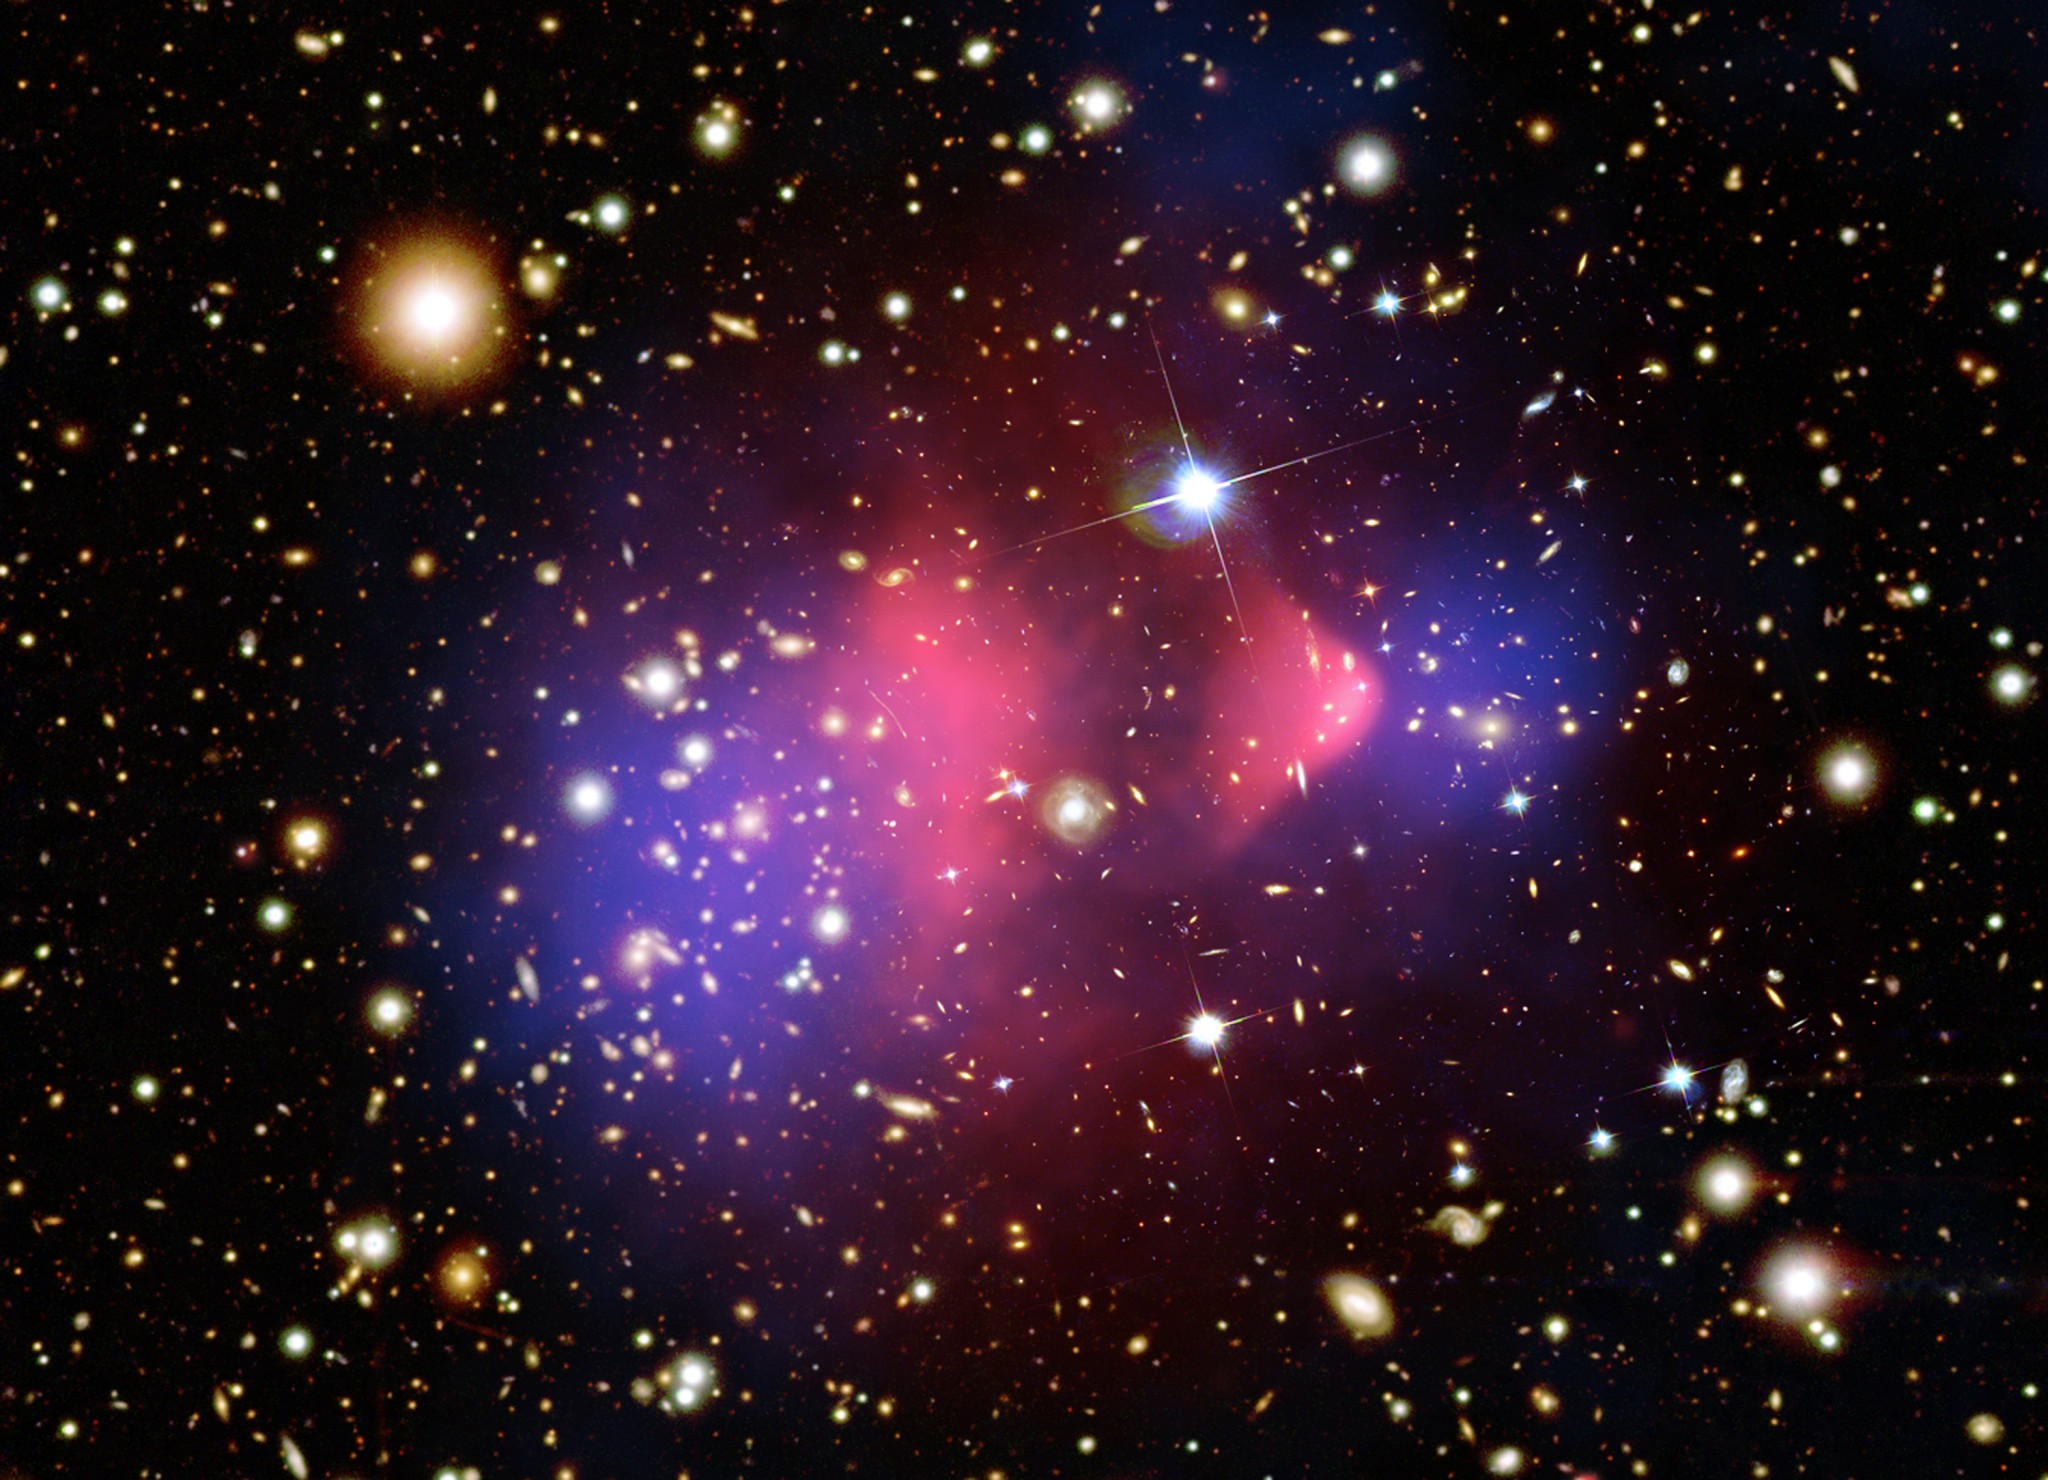
\includegraphics[width=0.95\textwidth]{images/bulletcluster.eps}
        \caption[The Bullet Cluster]{The bullet cluster\cite{bullet_cluster_combined_image}.  The blue clouds indicate the graviational lensing mass\cite{bullet_cluster}, the red represents two clouds of ionized baryons emitting x-rays\cite{bullet_cluster_chandramap}.  The remaining stars and galaxies are imaged in the optical spectrum\cite{bullet_cluster_composite}.}\label{fig:bullet}
      \end{center}
    \end{figure}

    Followup studies have also been done of other galaxy clusters.
    Mass to light ratios??


    In the second method, the velocity of different galaxies in a cluster can be measured.
    By comparing the velocities of different galxies in a cluster, the contained mass within the cluster can be measured.
    Mass to light ratios??

  \subsection{$10^{26}m$ : Universe Scale}
    %\subsection{Inter-Cluster Scale}
    % fast radio burst galaxy at z = 0.492 (http://www.nature.com/nature/journal/v530/n7591/full/nature17140.html)
    % redshift to distance : d = z c / Ho (http://m.teachastronomy.com/astropedia/article/Relating-Redshift-and-Distance)
    % wmap hubble constant = 70.4 (km/s)/Mpc (http://map.gsfc.nasa.gov/universe/bb_tests_exp.html)
    % c = 2.99*10^8 m/s = 2.99*10^5 km/s
    % 0.492 * 2.99*10^5 km/s / 70.4(km/s)/Mpc = 2089 Mpc = 6.44*10^25 m
    %?? NATURE PAPER IS IN QUESTION ??
    %At even larger scales of $\nicetilde 10^{25}$m, fast radio bursts and their frequency dispersion can be used to place limits on the amount of baryonic matter in the path of the burst.
    %This in turn allows for upper limits to be placed on the amount of dark matter present as well.
    %
    % age of universe (13.82*10^9 years * speed of light) = 1.307*10^26m
    At the largest scale of the universe, $\nicetilde 10^{26}$m, the cosmic microwave background (CMB) has been used to measure the total amount of dark matter in the universe.
    By looking at the structure of the CMB, earlier times in the universe can be studied.
    Closer to the big bang, there was a point in time referred to as the 'freezout'.
    Before that time, the universe was a sea of quark plasma and other particles, and the temperature was too hot to allow baryons exist for any long period of time.
    After that freezout time, the temperature low enough that baryons stopped being created and annihilated.
    Thus, the number of baryons that were in the universe at the freezout temperature determines how many baryons are in existance today, since there aren't any significant ways to destroy universe-scale quantities of baryons.
    This freezout left an imprint of its structure, where more baryons in some places created more CMB photons, and other places had less of each.

    From fitting this structure, the composition of the universe can be fit.
    In terms of energy, 69.1\% of the universe is composed of Dark Energy, which is causing almost all galaxies in sight to accellerate away from the Milky Way.
    Another 4.9\% of the universe's energy is stored in baryonic matter, like protons and neutrons.
    The remaining 26\% of the universe's energy is contained in Dark Matter\cite{planck2015}.

    As another important piece of evidence is the abundance of Deuterium present in the universe.
    The amount of deuterium that was left over from the big bang depends on the amount of baryons in the universe.
    The amount of baryons predicted by this is not enough to account for the total mass of the universe, thus it must exist in other (darker) particles.
    Most theories of dark matter being locked up in cold, dead stars (MACHOs) are limited by this baryon limitation (cite??).

    Another measurement that depends heavily on the presence of dark matter is the rate at which galaxies form clumps.
    In the Sloan Digital Sky Survey, which maps the positions of 1.6 million galaxies, quasars, and stars \cite{sdss_release}.
    By simulating the distribution of similar objects as the universe ages, only with a dark matter component does the universe form clumps that match SDSS observations.
    (reword/expand on this??)

\section{Indirect Dark Matter Detection}
  For this analysis, it is important to understand how a terrestrial telescope like VERITAS can detect the presence of dark matter.
  This is done through indirect detection: observation of the standard model particles that are emitted when two dark matter particles annihilate.
  As the rate of annihilation depends on the local dark matter number/volume density, the radially-changing structure of dark matter halos also affects the analysis.
  \subsection{WIMP properties}
    % relic cross-section?

    In the 1990s, it was pointed out that supersymmetry allowed for the existance of a WIMP-like particle with a crosssection of around \nicetilde 3 *  m.
    What also made this WIMP particle a promising candidate is a WIMP-like particle also solves several problems in cosmology, and that such a WIMP-like particle would have a similar cross section.
    Thus, two separate fields of physics came together and noticed that they both were looking for a WIMP-like particle within a mass and crosssection range.
    In $\Delta$CDM cosmology, the relic density is all of the lefover dark matter particles after the universe became too cold to produce more dark matter particles.
    (section needs more work??)

    There are other potential dark matter candidates, both as other particle types or as modifications to other areas of physics, but they are not explored in this thesis.
    see https://arxiv.org/pdf/1006.2483v2.pdf for more info??
  \subsection{Dark Matter and Gamma Rays}
    WIMPs are predicted to decay and self-annihilate into standard model particles.
    Primarily, indirect searches focus on annihilating WIMPs, as the predicted WIMP decay lifetime produces a lower standard model flux than annihilation(discuss more??).
    WIMPs may annihilate into any standard model particle, but most studies examine a WIMP annihilating into a quark-antiquark pair, or a pair of gamma-ray photons.

    For example, two annihilating WIMPs may produce a $\HepParticle{t}{}{}\HepAntiParticle{t}{}{}$ pair, which then decays into...??.
    Or, they may produce $\HepParticle{b}{}{}\HepAntiParticle{b}{}{}$, or $\HepParticle{\gamma}{}{}\HepParticle{\gamma}{}{}$.

    These different annihilations will produce different spectra of final gamma rays.
  \subsection{Dark Matter Halo Structure}
    From observations, most galactic dark matter halos can be modeled by several similar density profiles (explain??).
    Three of the primary profiles are the Burkert, the Einasto, and the Zhao profile.
    Each profile describes the mass/volume density of dark matter at a distance r from the halo center.

    A Burkert profile (\cite{burkertprofile}) has the form

    $ \rho_{DM} \left( r \right) = \frac{ \rho_o r_o3}{ \left( r + r_o \right) \left( r^2 + r_o^2 \right)} $ \label{eqn:burkert}

    where $r_o$ is the scale radius of the halo, and $\rho_o$ is the scale density, the density at the scale radius.

    The Einasto profile (\cite{einastoprofile1},\cite{einastoprofile2}) has the form

    $ \rho_{DM} \left( r \right) = Exp \left( - \frac{2}{\alpha} \left( {\left( \frac{r}{r_o} \right)}^{\alpha} - 1 \right) \right)$ \label{eqn:einasto}

    The Zhao profile (\cite{zhaoprofile}) has the form

    $ \rho_{DM} \left( r \right) = \frac{\rho_o}{ {\left( \frac{r}{r_o} \right)}^{\gamma} {\left( 1 + {\left( \frac{r}{r_o} \right)}^{\alpha} \right)}^{ \left(\beta - \gamma \right) / \alpha} } $ \label{eqn:zhao}

    where $\gamma$ is the slope of the density profile when $r << r_o$, $\beta$ is the slope when $r >> r_o$, and $\alpha$ determines how large the transition region is between $\gamma$ and $\beta$.
    A larger $\alpha$ means a smaller transition region.

    These profiles can then be used to calculate the spatial distribution of gamma-rays.
    For annihilating dark matter, $\rho\left(r\right)^2$ must be integrated along the line of sight.

    $ \frac{d\Phi}{dE d\Omega}= \frac{ \left \langle \sigma v \right \rangle }{8 \pi m_\chi^2} \frac{dN}{dE} \int \rho^2 dl $ \label{eqn:dmflux}

    ?? equation also depends on if particle is symmetric? 8 $\pi$ may change or something ??
    
    Additionally, some simulations of galaxy formation indicate that the presence of baryons diffuses (??) the central cusp of particles in a potential well (cite??).
    This create a central area of constant density in the profile called a core.
    So far, no studies have been able to determine whether a cored or cuspy profile is favored in observations.

    
  \subsection{Spectrum of Gamma Rays from Dark Matter}
    In order to calculate the brightness of the dark matter halo in gamma rays, the produced spectrum from each WIMP annihilation must be known.
    Each WIMP annihilation may directly produce two gamma rays, or may instead produce a $t\tbar$ or $b\bbar$ pair, which then decays into gamma rays (and other possible decay channels?? leptons??), called annihilation channels.
    In order to calculate the different produced gamma-ray spectra for each annihilation channel, the software package CLUMPY is used (cite??).

    For this thesis, only the simplest annihilation channels are considered, where WIMP annihilations only use one channel, instead of percent mixes of multiple channels.

    ?? plot of used spectra ??

    These spectra, then can be combined with the J-factor equation to calculate how many gamma rays are produced by the halo.

    ?? plot of j-factor with spectra ??


